% AER-Article.tex for AEA last revised 22 June 2011
\documentclass[AER,draftmode]{AEA}

\usepackage{graphicx}
\usepackage{apacite}
\usepackage[colorinlistoftodos]{todonotes}

\usepackage{setspace}


% The mathtime package uses a Times font instead of Computer Modern.
% Uncomment the line below if you wish to use the mathtime package:
%\usepackage[cmbold]{mathtime}
% Note that miktex, by default, configures the mathtime package to use commercial fonts
% which you may not have. If you would like to use mathtime but you are seeing error
% messages about missing fonts (mtex.pfb, mtsy.pfb, or rmtmi.pfb) then please see
% the technical support document at http://www.aeaweb.org/templates/technical_support.pdf
% for instructions on fixing this problem.

% Note: you may use either harvard or natbib (but not both) to provide a wider
% variety of citation commands than latex supports natively. See below.

% Uncomment the next line to use the natbib package with bibtex 
%\usepackage{natbib}

% Uncomment the next line to use the harvard package with bibtex
%\usepackage[abbr]{harvard}

% This command determines the leading (vertical space between lines) in draft mode
% with 1.5 corresponding to "double" spacing.
\draftSpacing{1.5}
\setlength{\marginparwidth}{4cm}
\setlength{\parskip}{1em}

\begin{document}

\title{Does Coverage of Sexual Assault Cases Ease the Reporting Decision? Evidence from FBI Data}
\shortTitle{Sexual Assault Reporting}
\author{Harry Elworthy\thanks{Duke University, harryelworthy@gmail.com.}}
\date{\today}
\pubMonth{}
\pubYear{}
\pubVolume{}
\pubIssue{}
\JEL{}
\Keywords{}

\begin{abstract}
Your abstract here.

Files available at \url{github.com/harryelworthy/Thesis}
\end{abstract}


\maketitle

%American Economic Review Pointers:

%\begin{itemize}
%\item Do not use an "Introduction" heading. Begin your introductory material
%before the first section heading.

%\item Avoid style markup (except sparingly for emphasis).

%\item Avoid using explicit vertical or horizontal space.

%\item Captions are short and go below figures but above tables.

%\item The tablenotes or figurenotes environments may be used below tables
%or figures, respectively, as demonstrated below.

%\item If you have difficulties with the mathtime package, adjust the package
%options appropriately for your platform. If you can't get it to work, just
%remove the package or see our technical support document online (please
%refer to the author instructions).

%\item If you are using an appendix, it goes last, after the bibliography.
%Use regular section headings to make the appendix headings.

%\item If you are not using an appendix, you may delete the appendix command
%and sample appendix section heading.

%\item Either the natbib package or the harvard package may be used with bibtex.
%To include one of these packages, uncomment the appropriate usepackage command
%above. Note: you can't use both packages at once or compile-time errors will result.

%\end{itemize}

\clearpage
\section{Introduction}

An estimated 18.3\% of women and 1.4\% of men in the United States are sexually assaulted at some point in their lives, with more than a third of these assaults occurring before the victim turns 18  \cite{black_national_2011}. About 20\% to 25\% of women nationally are sexually assaulted at some point during their college careers \cite{fisher_sexual_2000}. At Duke, this figure is estimated at closer to 40\%, as well as 10\% of men \cite{fox_university_2017}. Despite this, very few assaults are reported to police. According to \citeA{fisher_sexual_2000}, "fewer than 5\% of attempted or completed sexual assault against college age women are reported to law enforcement. 66\% of victims tell friends but not family or school officials." \citeA{resnick_predictors_2000} finds that 1/5 of women that experience sexual assault report it to police, while \citeA{greenfield_sex_1997} estimates this number at 1/3 of women. Because these studies use self-reported survey data, there are still almost certainly non-reporting women and thus these estimates are likely upper bounds. Victims do not report to police for a number of reasons, discussed more in-depth below, including self-blame, guilt, fear of the perpetrator or fear of not being believed \cite{du_mont_role_2003}.

There are many reasons to seek to increase the proportion of sexual assaults that are reported. Some victims of of sexual assault do not want to report their crime to police because they do not wish their perpetrator to face justice, often because they are friends or are otherwise close. However, many victims would prefer to report their crime to the police, and balance this desire against the costs they see in reporting, costs summarized above and discussed in more depth below\todo{Need a source here}. There also obviously cannot be a criminal investigation if the crime is not reported to the police, and so women may wish to report in order to see justice for their assaulter. Victims of rape that report the crime to the police are also 9 times more likely to receive medical care than those that do not \cite{resnick_predictors_2000} as well as more likely to receive psychological care \cite{sable_barriers_2006} meaning that it is often in the interest of the victim's health for them to report the crime to police. Equally, there is a benefit to society of reporting. \citeA{bachman_factors_1998} notes that "an unreported incident of rape eliminates the possibility that an offender will be arrested or convicted. This may, in turn, reduce the perceived likelihood that rape and sexual assault, in general, will be punished." This reduction in perceived likelihood of punishment has significant consequences. A number of studies have found that the propensity of men to commit sexual assault is significantly decreased by the threat of formal sanctions such as arrest \cite{bachman_rationality_1992, antunes_impact_1974}. Additionally, \citeA{abel_self-reported_1987} finds that non-incarcerated rapists have high recidivism rates, suggesting that unreported assaults pose a serious threat to others. Finally, increased reporting can be a sign that the barriers to reporting that victims feel, barriers often steeped in misogyny, are declining in severity. This is surely a thing to strive for.

Previous research has focused on many factors affecting the reporting decision, including relations of the victim to the perpetrator, whether the act was violent, whether alcohol was involved, and much more. This research is discussed more thoroughly in the next section. One factor not previously investigated, however, is the response of reporting behaviour to prominent coverage of sexual assault allegations and cases. The \#metoo movement that the Harvey Weinstein allegations started focused on women coming forward with their sexual assault stories because they saw others come forward with theirs - thus the 'me too.' This idea highlights an important question: are victims of sexual assault encouraged to report to police or other authorities by coverage of other victims reporting?

In this paper, I explore these questions using incident-level FBI data of crime reports from 2008 to 2016, along with search-volume data from Google Trends. I supplement this  with instrumental-variable analysis using a novel dataset of high-profile sexual assault allegations. 

\section{Background}

Since Becker outlined his economic model of crime, illicit activities have continued to have a place in the economic literature. Sexual assault has received a share of this attention, although perhaps less so than other crimes. One reason for this deficit is the difficulty of gathering accurate data on sexual assault. Crime is under-reported in general, sexual assault especially \cite{fisher_sexual_2000}. This under-reporting makes the study of sexual assault inherently difficult, because no study will ever be able to accurately gauge how many assaults actually occurred over a given time period. Studies that use surveys to estimate this under-reporting are always subject to under-reporting of their own, as even simply answering a survey question about sexual assault is difficult for many victims \cite{du_mont_role_2003}. When observing an increase in reports, the inability to observe assault numbers also creates issues of inference. Are reports increasing because people feel more safe reporting their assaults, or because assaults themselves are increasing? Different papers approach these issues in different ways when dealing with sexual assault.

Recently, several papers in economics have focused on sexual assault and harassment. \citeA{lindo_college_2018} looks at the effect of partying culture on reports of sexual assault using the plausible exogeneity of Division 1 football games. The authors find a 28\% increase in rape reports associated with game days.\footnote{This paper also uses the FBI incident-level data, and I use their code in my analysis.} \citeA{bisschop_street_2017} investigates the effect of opening a 'Tippelzone,' an area of a city where street prostitution is legalized, on reported sexual assaults. Using a difference-in-difference approach across different cities, the authors find decreases in registered sex crime of 30 to 40\% in the two years after the zone is opened. Depending on the type of zone, there are also decreases in associated crimes such as crimes related to drugs. \citeA{borker_safety_2018} investigates how perceived risk of street harassment affects women's human capital attainment, finding that women are willing to spend twice the annual cost of tuition of a university for a route to university that is perceived to be one standard deviation safer from sexual harassment, and to attend worse universities to increase their perceived safety.

Only one recent economics paper focuses on the decision for a victim of sexual assault to report: \citeA{allen_reporting_2007} investigates the factors that influence an individual's decision to report a rape to law enforcement using survey data from the National Crime Victimization Survey and finds that victims will be more likely to report sexual assault given more 'social support' as well as if the victim has ancillary evidence associated with the crime. The author defines a number of variables as contributing to each of these categories. The victim being married, their offender being a stranger, their neighborhood being predominantly divorced households or households that have lived in the area for more than five years, and the victim's family income are all considered as factors that contribute to 'social support' for the victim, and each increase the propensity for a victim to report.

More attention is paid to the reporting decision by other fields, especially law. A number of studies find that a victim's propensity to report is increased when the offender uses physical force \cite{bachman_predicting_1993,du_mont_role_2003}. This is likely because of both a desire to receive medical care - as seen above, those that report their assault to the police are much more likely to receive medical care than those that are not - and because physical violence often provides the victim evidence of the crime. \citeA{bachman_predicting_1993} also investigates whether the reporting decision is affected by the relation of the victim to the offender or by whether the event occurred at the victim's house, but finds no significant effects. All of these studies use the same National Crime Victimization Survey data for their studies, over different periods of time. Other survey-style studies exist too. \todo{Need to grab them from bachman references.}

These studies have their limitations. Because they all use self-reported surveys, they suffer from some sort of selection bias, in that there will always be people that are asked but do not participate. There will also always be people that report things incorrectly. In the case of sexual assault surveys, there are very likely victims that do not report their assault even to surveyors because doing so may be traumatic. This selection bias and misreporting is a problem that is very hard to avoid in a survey-style study, because there is no way to know if the characteristics of these people are the same as those that fill out the survey accurately. Consider an example. Suppose people who are violently assaulted but do not report their assault to police are ashamed of their non-reporting, and so when asked by surveyors they say they have never been assaulted. This behavior would undermine the results of \citeA{bachman_predicting_1993}, i.e. that victims report to police more often when their assault involves violence, because we cannot see the non-reporters of violent attacks. In addition to this, these studies tend to struggle to convincingly infer causality. As an example, \citeA{du_mont_role_2003} concludes that women that visit the hospital after an assault are more likely to report their assault to the police. \citeA{resnick_predictors_2000}, using the same dataset, concludes that women that report their assault to the police are more likely to receive medical care. Because these studies use single time period survey data, there is no simple way to solve this issue of causality.

My paper aims to contribute to the literature by considering the effect that national coverage of sexual assault cases and allegations have on sexual assault reporting. This research question is interesting because it has not been approached before, but also because it lends itself to a different type of analysis: time-series and instrumental variable analysis of FBI data of actual reports to police. This data would not be able to answer many of the questions above because it does not have the detailed information that the NCVS has on victims, nor does it have any indication of victims that do not report. However, for something like news coverage, which I measure at a national level and for which a number of exogenous shocks can be identified, the FBI data works well. By using actual reports to police instead of reports and non-reports to police from survey data, I am able to escape the issue of selection-bias \todo{Explain why}. I am also able to address causality more clearly, through instruments using exogenous shocks \todo{and just the fact that causality in one direction is just likely much stronger}. There are clear limitations to my approach as well, which I discuss in my conclusion section, but it does avoid many of the problems discussed above.

This question of the effect that news coverage has is important. Most important is its sign, because a negative effect of news coverage could have serious police implications. If research found that coverage of sexual assault cases had a significant deppresing effect on the reporting of new sexual assaults, this might be cause for policy either within the media industry or from government to reduce such coverage. An allegory that comes to mind is the coverage of suicide cases. It is well established that media coverage of suicide tends to have a copycat effect \cite{stack_media_2003}. This is undesirable for a society that wishes to minimize loss of life, and so many countries such as New Zealand, Australia and Canada have strict guidelines on how the media can report on suicide. In the US, there are a number of organizations that advocate for reduced and more careful reporting of suicide \cite{noauthor_reportingonsuicide.org_2019}. If reporting on sexual assault produced the opposite of a copycat effect, i.e. it stopped people from reporting their assaults, one might be incline to recommend similar policy for the coverage of sexual assault cases. \todo{Need some reason that it's still interesting if positive!!}

Previous economic research has used search volume in similar ways.
\begin{itemize}
    \item Needed! Have close to nothing here
\end{itemize}

\section{Data Summary}

I have two main data sources for this project: The National Incident-Based Reporting System (NIBRS) and relative search volumes from Google Trends. The NIBRS has data on individual reports of crime to police stations, from 1991 to 2016. About 25\% of the population is covered, as some states only report summary statistics while others do not give data at all. This percentage increased since 1991 as more stations have begun reporting. There are timestamps for both report and incident date and time, and the data includes some auxiliary information about the victim in question, including their age, race, and whether the incident involved alcohol. Because the data is by incident, it can be collapsed to any specification: nationally daily, by state, etc. When collapsing, I remove from each day incidents that were both reported and occurred that day - i.e. I only keep reports of events from before the day in question. In this way, I hope to avoid findings that include shifts in assaulting behavior from coverage of sexual assault cases, and only include shifts in reporting behavior. 

The data from Google Trends is relative search volume of a given term, scaled so that 100 is the highest volume over that time period. I collect data in six month periods, as this is required to get daily values, and then scale the data to the values in the first half of 2008 using values from overlapping dates. I use the search term “sexual assault”.\footnote{I decided on "sexual assault" as "rape" tended to have a lot of unsavoury related searches, mostly pornography related, whereas searches for sexual assault tended to be related to cases of sexual assault. "rape" also tended to be a lot noisier than "sexual assault" around times of a high profile sexual assault case} Google Trends can provide data nationally or by state, and I use both in my analysis. I merge the two datasets by day for national data and by day and state for state data.

I'd like to have a small table of summary statistics here.

\section{Methodology}

I spend the first half of this section looking at this decision from a theoretical perspective, and consider why news coverage of sexual assault cases and allegations could be a cost or a benefit. The second half details my empirical methodology.

The decision to report can be considered as a probabilistic decision that factors in both costs and benefits of reporting \cite{allen_reporting_2007}. Consider the simple model of the decision a victim makes:

$$
P(report_t) = \beta_0 + \beta_1 coverage + \varepsilon
$$

Where $report_t$ is a binary indicator of whether the victim will report their assault to the police in time period $t$, $coverage$ is a measure of news coverage of sexual assault related news - in my case, approximated with Google search volume - and $\varepsilon$ is an error term that includes other factors that might affect the decision to report, such as relation to the perpetrator or whether the event was violent. This paper hopes to estimate the sign of $\beta_1$ by considering the effect of coverage on total report numbers. 

It is not clear what we should expect the sign of $\beta_1$ to be. Coverage of sexual assault stories might decrease the social stigma that victims see associated with reporting a sexual assault, and thus ease the reporting decision for them. It might inspire victims to see other victims step forward. It might simply remind victims that they can report their assualt as a crime. These ideas are what lie behind the \#metoo movement, where a high-profile set of allegations against Harvey Weinstein encouraged a number of other victims to come forward and discuss their assaults. However, we might expect effects in the other direction too. Victims might see the way that prominent reporters of sexual assault are treated - for example, the flurry of derision directed at Christine Blasey Ford by those in even the highest seats of power - and conclude that the costs of reporting are higher than they initially thought. They might feel that reporting their assault in the wake of a high profile case could reduce the chance of people believing them. \todo{Any other reasons?}

The data that I use allows the examination of subgroups by age, race and by whether the incident involved alcohol, so it is worth considering how we might expect effects to vary across these categories. Regardless of the sign of effect, we might expect the magnitude to be greater for younger than for older victims for a number of reasons. Young people are bigger consumers of media than older people \todo{Need source} and so might be more likely to read about prominent allegations in the news. It also seems reasonable to assume that for any of the possible effects discussed above, magnitudes would diminish after the first time a victim saw coverage related to sexual assault. \todo{Is there another reason that older people might not find it? Might not find inspiration/less optimism about the process/something?} There is no clear prediction to be made about how the effect might vary across races. One might expect the effect to be more positive among incidents that don't involve alcohol than those that do, as in those events the victims generally have greater ancillary evidence \cite{allen_reporting_2007}, although this prediction is not very strong. \todo{In general need this to be worded much better and include more evidence from other papers.}

A significant issue with this type of study is that I have no sense of how numbers of actual assaults are changing over time. This could mean that an increase in reports of sexual assaults is being driven by an increase in the reporting of assaults or the number of actual assaults. These two outcomes would have very different meanings and would lead to very different policy responses. It is thus very important to attempt to correct for this. I attempt to do this in my paper by dropping all events whose incident and report-dates are the same - that is, events that are reported on the day that they are committed. Using this measure of reports, if we see high search volume days having high numbers of reports, it is reasonable to assume that the increase is not being driven by increases in actual assaults (as these assaults would have had to happen during the high trend, i.e. on that day, and thus they would not have been counted). This is not a perfect correction. Many incidents only have report dates, presumably because the victim wasn't sure or didn't want to report the date that the incident occurred on \todo{Include percentage that do/don't}. Some of these may have occurred on the day they were reported, and so my strategy of deletion may not be complete.

In order to estimate the sign and magnitude of $\beta_1$ discussed above, I run a series of time series regressions and supplement these results with instrumental variable analysis. My initial regressions are time series regressions at the daily level, and are of the form: 

$$ 
y_{t} = \beta_{0} + \sum_{b=-7}^{7} \delta_{b} x_{t+b} + \gamma_{t} + \varepsilon_{t}
$$

Where $y_{t}$ is the outcome variable in question; $x_{t+b}$ is the independent variable in question along with a set of leads and lags, and $\gamma{t}$ is a vector including day-of-week, week-of-year and year fixed-effects. These fixed effects should take care of most seasonality in the data. I include 7 leads and lags as a way to account for events happening in close proximity to each other without reducing degrees of freedom unnecessarily.

To accompany these time series results, I find events that are plausibly exogenous shocks to the volume of coverage of sexual assault-related topics, and use these shocks to instrument for the effect of an increase in such coverage on numbers of reports of sexual assault. These events are collected using Google's "Related Queries" function, that collects searches that are made in conjunction with the term in question over a specified time period. I look at times at which the Google Trend for 'sexual assault' is above 60\% of its 6-month maximum for the 9 years in question, which gives 563 days. For each day, I look for distinct related queries. For example, on November 19, 2014, 'Bill Cosby' is the top related query, as he is for the next several days. I count only the first occurrence of these terms as a distinct 'high profile event.' To use these events as instruments for the Google Trend, they must be correlated with the Google Trend and uncorrelated with the error term. I analyse the first requirement in the results section. 

The second requirement - that these events are uncorrelated with the error term - requires some qualitative justification, as components of the error term are inherently unobservable. This requirement can be reworded as: high profile events cannot affect report rates through any avenue except through intensity of news coverage, here measured by search volume. Is it possible that these events affect reporting in other ways? I argue that it is not likely in any significant way. It is possible that these events themselves involve reports to police on the days of news coverage - i.e. that an accuser of a prominent case would report to the police and this would be counted in that day's reports - but this could not contribute in any significant way to total daily reports, given that more than 100 reports of rape are filed every day. Any other avenue \todo{Need better word, there's an econ word for this. Need another example of an avenue too.} would likely be caught in the proxy of search volume. Thus this assumption about the instrument seems valid.

I use these events in a number of two stage least squares regressions. To take advantage of the 3 day window of significant effects on the Google Trend and reduce the standard errors of results, I bin results into the three day period including the event and two lag variables. I use two different methods of two-stage least squares regressions to obtain results. The first uses a binary variable $event\_bin$ as the instrument, which is 1 if a high-profile event occurred in the past 3 days and 0 otherwise. The second uses dummy for each individual event's bin as the instrument. This means that while the first method obtains an estimate using the variation in trend and reports between event- and non-event- dates, the second uses the variation between events. I shall refer to these as IV Specification 1 and IV Specification 2 for the rest of the paper.  \todo{Outline here the first stage (different for each?) and the second stage, in equations}

The first stage for the first IV specification is thus modeled as:

$$ 
trend_{t} = \delta_{0} + \delta_1 event\_bin_t + \epsilon_{t}
$$

And for the second IV specification is modeled as:

$$ 
trend_{t} = \delta_{0} + \delta_1 events\_factor_t + \epsilon_{t}
$$

Where $events\_factor$ is a vector of dummy variables for each individual event. The second stage for both regressions is then:

$$ 
reports_{t} = \beta_{0} + \beta_1 \hat{trend} + \varepsilon_{t}
$$

Where $\hat{trend}$ is the predicted values of the given first stage. \todo{Add in fixed effects where they are used}

To consider variation by state, I run a panel regression of the form:

$$ 
reports_{i,t} = \beta_{0} + \sum_{b=-7}^{7} \delta_{b} trend_{i,t+b} + \alpha_{i} + \gamma_{t} + \varepsilon_{i,t}
$$

Where $reports_{i,t}$ are reports in state $i$ on date $t$; $trend_{i,t+b}$ is the relative search volume in state $i$ on date $t$ along with a set of leads and lags, $\alpha_{i}$ is a fixed effect at the level of the state, and $\gamma{t}$ is a vector including year fixed-effects, day-of-week and week-of-year fixed effects. \todo{All results section needs to be changed to log form}

\section{Results}

I begin by running a time-series regression of reports of sexual assault to the FBI by report-date on national Google Trends for 'sexual assault'\todo{How best to note that it is in log form? once at the start? In every graph, in axes, in title?}. The results of this are shown in Figure~\ref{figure:police_trends_daily_logboth}. There is a clear, statistically significant effect on the first lag variable. I show this effect, as well as the same effect broken down by subgroups of age and race of the victim and whether the event was reported as involving alcohol, in the first column of Table~\ref{table:combinedtable}. 

To complement this time series analysis, I perform the same subgroup analysis with two different instrumental variable specifications as discussed in the methodology section. 

To test the effect of these 'high profile events' on the Google Trend, I graph the response of the Trend before and after an event takes place, including fixed effects for year, week of year and day of week. This is shown in Figure~\ref{figure:events_trend}. As can be seen, these events have sizable effects on the Google Trend for 'sexual assault' that last for about 3 days. Thus they look to be good examples of random positive shocks to the google trend. To check whether reports seem to be impacted by these events occurring, I look at reports to police before and after these events in three day bins, including the same fixed effects as above. This is shown in Figure~\ref{figure:events_police_binned}. We see that reports do indeed increase around the date of an event, albeit with large standard errors.  The results of the instrumental variable regressions are shown in columns 2 and 3 of Table~\ref{table:combinedtable}. 

\begin{figure}
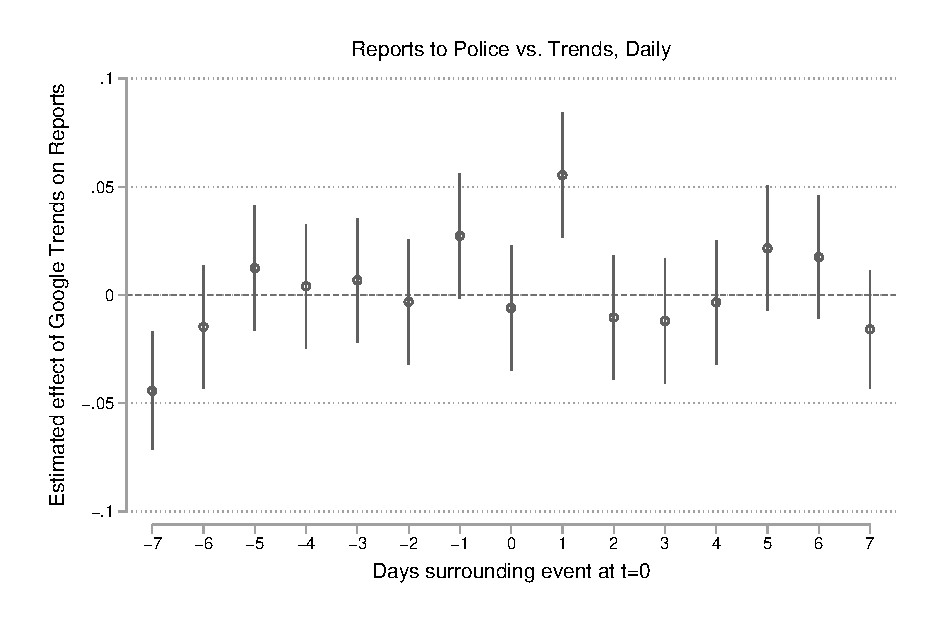
\includegraphics[width=\linewidth]{figures/police_trend_daily_logboth.eps}
\caption{Time-Series Regression of FBI Reports of Sexual Assault on Google Trends for 'sexual assault'} \label{figure:police_trends_daily_logboth}
\end{figure}

\begin{table}[]
\caption{Combined results of effect of increases in Google Trend on reports of sexual assault} \label{table:combinedtable}
{
\def\sym#1{\ifmmode^{#1}\else\(^{#1}\)\fi}
\begin{tabular}{l*{3}{c}}
\hline\hline
            &\multicolumn{1}{c}{(1)}&\multicolumn{1}{c}{(2)}&\multicolumn{1}{c}{(3)}\\
            &\multicolumn{1}{c}{log\_reports}&\multicolumn{1}{c}{log\_reports}&\multicolumn{1}{c}{log\_reports}\\
\hline
log\_trend   &      0.0568\sym{***}&       0.901\sym{*}  &      0.0521         \\
            &    (0.0146)         &     (0.434)         &    (0.0913)         \\
\hline
log\_trend\_10\_to\_19&      0.0611\sym{**} &       0.149         &     -0.0693         \\
            &    (0.0190)         &     (0.168)         &     (0.120)         \\
\hline
log\_trend\_20\_to\_29&      0.0315         &      0.0740         &      0.0104         \\
            &    (0.0196)         &     (0.169)         &     (0.129)         \\
\hline
log\_trend\_30\_to\_39&      0.0405         &      0.0109         &       0.226         \\
            &    (0.0280)         &     (0.240)         &     (0.176)         \\
\hline
log\_trend\_40\_to\_49&     -0.0324         &      -0.126         &      -0.471\sym{*}  \\
            &    (0.0369)         &     (0.315)         &     (0.223)         \\
\hline
log\_trend\_50\_to\_59&      0.0408         &       0.343         &       0.273         \\
            &    (0.0446)         &     (0.377)         &     (0.250)         \\
\hline
log\_trend\_60\_to\_69&      0.0320         &       0.179         &      -0.120         \\
            &    (0.0468)         &     (0.482)         &     (0.259)         \\
\hline
log\_trend\_white&      0.0578\sym{***}&       0.160         &       0.122         \\
            &    (0.0153)         &     (0.135)         &    (0.0970)         \\
\hline
log\_trend\_black&      0.0645\sym{**} &      0.0179         &     0.00573         \\
            &    (0.0233)         &     (0.201)         &     (0.140)         \\
\hline
log\_trend\_other&      0.0389         &      -0.122         &      -0.728\sym{**} \\
            &    (0.0408)         &     (0.353)         &     (0.274)         \\
\hline
log\_trend\_alc&     -0.0176         &     -0.0565         &      -0.195         \\
            &    (0.0530)         &     (0.260)         &     (0.271)         \\
\hline
log\_trend\_non\_alc&     -0.0176         &     -0.0565         &      -0.195         \\
            &    (0.0530)         &     (0.260)         &     (0.271)         \\
\hline
\(N\)       &        3288         &        3289         &        3289         \\
adj. \(R^{2}\)&       0.273         &           .         &       0.190         \\
\hline\hline
\multicolumn{4}{l}{\footnotesize Standard errors in parentheses}\\
\multicolumn{4}{l}{\footnotesize \sym{*} \(p<0.05\), \sym{**} \(p<0.01\), \sym{***} \(p<0.001\)}\\
\end{tabular}
}

\end{table}

\begin{figure}
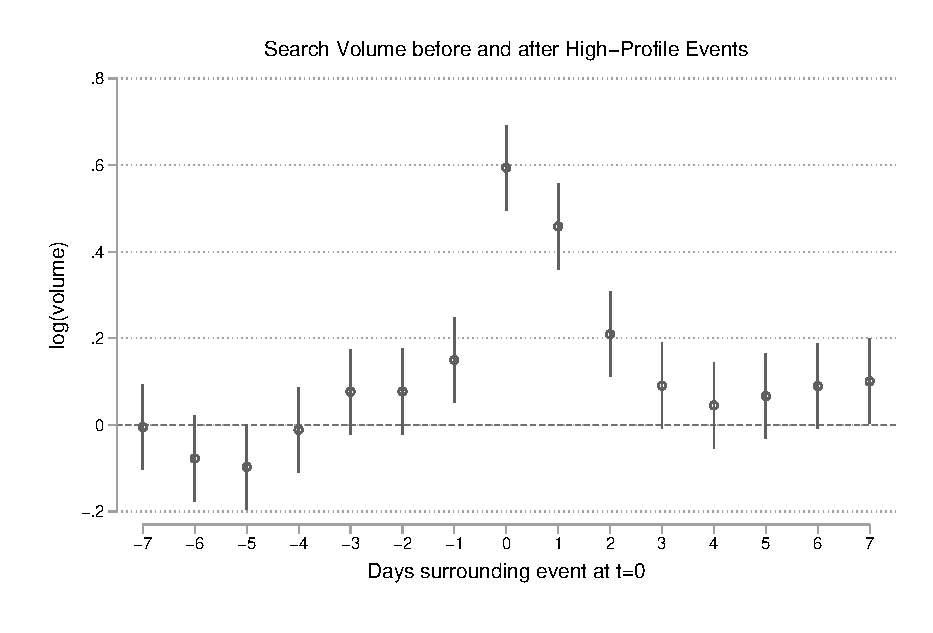
\includegraphics[width=\linewidth]{figures/events_trend.eps}
\caption{Google Trends before and after High Profile Events} \label{figure:events_trend}
\end{figure}

\begin{figure}
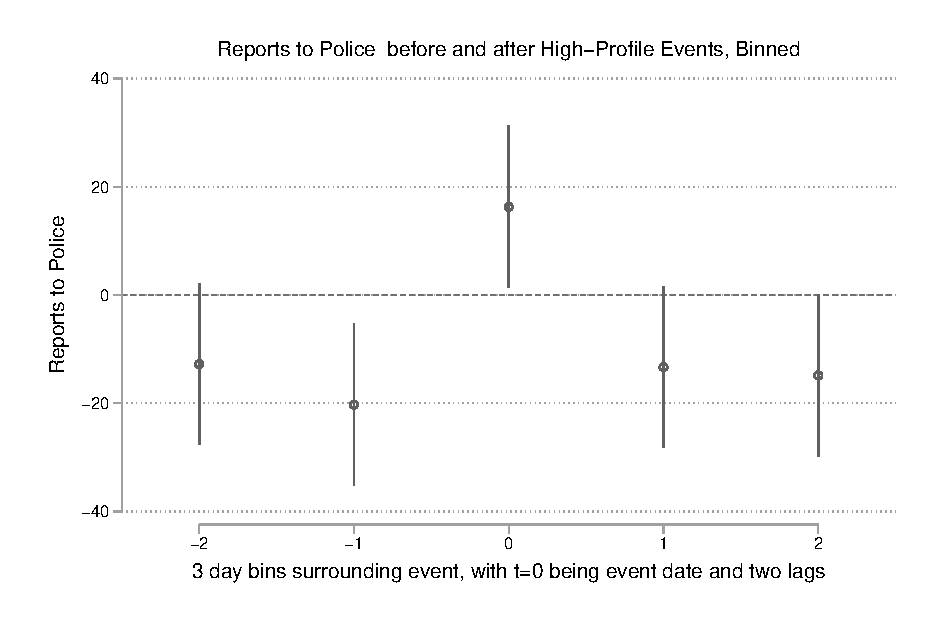
\includegraphics[width=\linewidth]{figures/events_police_binned.eps}
\caption{Reports to the FBI before and after High Profile Events, Binned} \label{figure:events_police_binned}
\end{figure}

All three specifications give positive coefficients for the overall effect, ranging in magnitude from 0.0568 to 0.219. To contextualize this, the mean daily number of reports per day from 2008 to 2016 was 110. \todo{Would median be more appropriate here?} According to the low estimate, a 1\% increase in the search volume for 'sexual assault' for a day leads to an increase of 0.062 reports, while the high estimate gives an increase of 0.24 reports. Given that the NIBRS data only covers 1/4 of the US, if we assume a homogeneous effect across the country, these estimates become 0.25 and 0.96 reports respectively.

To give further context, the increases in search volume depicted in Figure~\ref{figure:events_trend} give an average increase in search volume of 42\% over the day of the event and the two days following. Given these increases, one of these events occurring will result in a spike of between 31 and 121 reports nationally, according to my low and high estimates respectively. For events where the google trend was above 80\% of the 6-month maximum for 3 days (i.e. very large events), these estimates are 46 and 178 reports nationally.

This increase appears to be driven by young reporters, as predicted above. Depending on the specification, there is also a significant effect (higher than the effect for young people) among reporters over 50, something non hypothesized. All specifications agree on only small positive or even some negative effects for victims between 20 and 50, although none of the effects are statistically significant. White reporters increase more than average under all specifications, and for the naive time series so do Black reporters, although the IV models fail to find significance here. Events with no alcohol involved increase at greater rates than average for all models, with events involving alcohol having null effects. There are, however, significant limitations with this sub-group analysis. As in the summary statistics table, most victims are young, white and reporting events that did not involve alcohol. It is perhaps not surprising, then, that these are the categories where we find statistical significance. Without more observations, it is difficult to say whether we are seeing differences in groups or simply large standard errors for subgroups with lower numbers of observations.

I next look at variation in effect by state, to try to determine whether states with relatively higher trends on a given day have higher numbers of reports. \todo{Bad sentence here} I consider this using the  panel regression outlined above. Results are shown in Table~\ref{table:state_daily}. I fail to find significant results, indicating that coverage at a more local level may not have the effects that national coverage does. Again, however, this may be a case of individual states not having enough observations to give significance.

\begin{table}[]
\caption{Effect of increases in state Google Trend on reports of sexual assault} \label{table:state_daily}
{
\def\sym#1{\ifmmode^{#1}\else\(^{#1}\)\fi}
\begin{tabular}{l*{1}{c}}
\hline\hline
            &\multicolumn{1}{c}{(OLS)}\\
            &\multicolumn{1}{c}{log\_reports}\\
\hline
log\_trend   &    -0.00422         \\
            &    (0.0289)         \\
\hline
\(N\)       &        6676         \\
adj. \(R^{2}\)&      -0.300         \\
\hline\hline
\multicolumn{2}{l}{\footnotesize Standard errors in parentheses}\\
\multicolumn{2}{l}{\footnotesize \sym{*} \(p<0.05\), \sym{**} \(p<0.01\), \sym{***} \(p<0.001\)}\\
\end{tabular}
}

\end{table}

To consider whether assaults reported during high-coverage times are different in nature to those reported during low-coverage times, I run the same three specifications as above, but use $percent\_arrest_t$ as the dependent variable, where $percent\_arrest_t$ is the percentage of incidents reported on date $t$ that resulted in arrest. The results are shown in Table~\ref{table:arrest}. All three specifications give negative coefficients but fail to reject the null, indicating

\begin{table}[]
\caption{Effect of increases in Google Trend on percent of reports resulting in arrest} \label{table:arrest}
{
\def\sym#1{\ifmmode^{#1}\else\(^{#1}\)\fi}
\begin{tabular}{l*{3}{c}}
\hline\hline
            &\multicolumn{1}{c}{(1)}&\multicolumn{1}{c}{(2)}&\multicolumn{1}{c}{(3)}\\
            &\multicolumn{1}{c}{percent\_arrest}&\multicolumn{1}{c}{percent\_arrest}&\multicolumn{1}{c}{percent\_arrest}\\
\hline
log\_trend   &     -0.0234         &     -0.0203         &    -0.00684         \\
            &    (0.0143)         &    (0.0481)         &    (0.0343)         \\
\hline
\(N\)       &        1461         &        1461         &        1461         \\
adj. \(R^{2}\)&       0.023         &       0.013         &       0.015         \\
\hline\hline
\multicolumn{4}{l}{\footnotesize Standard errors in parentheses}\\
\multicolumn{4}{l}{\footnotesize \sym{+} \(p<0.10\), \sym{*} \(p<0.05\), \sym{**} \(p<0.01\), \sym{***} \(p<0.001\)}\\
\end{tabular}
}

\end{table}

\clearpage
\section{Conclusion}

Then spend some time discussing a similar thing but for potential perpetrators - expected cost of assault. Obviously even more than the other one this is a behaviour that is tough to rationalize, but it's not wild to think (and one would seriously hope) that at the margin these people can be influenced one way or another

Talk about the two in tandem, and again why hopefully reporting affects the second, and thus is important. If possible, this link would be great to try to estimate, but very difficult given the nature of the data. 

Discuss whether any of these might be false reports. Hopefully have data to back it up.

Discuss how this may be people coming forward more quickly, not just new reports, which are still interesting but not as meaningful.

Discuss potential next steps.


% The appendix command is issued once, prior to all appendices, if any.
\clearpage
%References here (manual or bibTeX). If you are using bibTeX, add your bib file 
%name in place of BibFile in the bibliography command.
% Remove or comment out the next two lines if you are not using bibtex.

\bibliographystyle{apacite}
\bibliography{refs}

\clearpage
\appendix

\begin{table}[]
\caption{High Profile Events, collected using Google Related Trends on high-trend days}
{
\def\sym#1{\ifmmode^{#1}\else\(^{#1}\)\fi}
\begin{tabular}{llr}
\hline\hline
date       & name                                  & big\_event \\
\hline
21/07/2009 & Roethlisberger                        &            \\
09/03/2010 & Roethlisberger                  &            \\
30/09/2010 & MSU Athletes                          &            \\
22/11/2010 & Notre Dame Suicide  &            \\
16/02/2011 & Lara Logan   &            \\
29/11/2011 & Wellesley    &            \\
10/01/2012 & Joe Philbin son                       &            \\
01/04/2012 & SA Aware Month                        &            \\
15/05/2012 & Prosper TX athlete                    &            \\
18/10/2012 & Amherst Document                      &            \\
28/12/2012 & Case McCoy                            &            \\
19/01/2013 & Michael Crabtree                      &            \\
01/04/2013 & SA Aware Month                        &            \\
07/05/2013 & USAF                          &            \\
14/11/2013 & Jameis Winston                        & 1          \\
01/05/2014 & 55 colleges sexual assault            &            \\
10/09/2014 & Jerry Jones            &            \\
19/11/2014 & Bill Cosby                            & 1          \\
27/02/2015 & Scott Walker                          & 1          \\
25/03/2015 & Lara Logan           &            \\
27/03/2015 & Subway            &            \\
01/04/2015 & Bikram Choudhury                 &            \\
15/04/2015 & Panama City                      &            \\
21/05/2015 & Josh Duggar                           &            \\
21/09/2015 & College Climate paper released        &            \\
09/11/2015 & Biden Speech                            &            \\
23/11/2015 & Jameis Winston                 &            \\
02/12/2015 & James Deen                            &            \\
30/12/2015 & Bill Cosby                      & 1          \\
07/01/2016 & Cologne New Year Assaults             &            \\
12/01/2016 & David Bowie                           &            \\
13/02/2016 & Peyton Manning                        & 1          \\
29/02/2016 & Lady Gaga                             & 1          \\
01/04/2016 & SA Aware Month                        &            \\
13/04/2016 & Kobe Bryant                           &            \\
10/06/2016 & Stanford Student                      & 1          \\
08/10/2016 & Donald Trump                    & 1          \\
\hline\hline \\
\end{tabular}
}
\end{table}


\end{document}

